\section{连续}

本节给出的函数连续的定义,并给出连续的运算和定理。
最重要的是根据定理推导的一个重要的极限。

本节要点:
\begin{itemize}
    \item 理解连续的概念;
    \item 推导一个重要的极限:$\underset{x\rightarrow 0}{\lim}\frac{a^x-1}{x}=\ln a$。
\end{itemize}

%============================================================
\subsection{连续的概念}

\begin{definition}[连续]
设$f\left( x \right) $在某邻域$N\left( x_0 \right) $内有定义,若
\[
\underset{x\rightarrow x_0}{\lim}f\left( x \right) =f\left( x_0 \right)
\]
则称{\bf $f\left( x \right) $在点$x_0$处连续(continuity)}。
\end{definition}

连续在数学上规范了什么是“不断”。

\begin{definition}[区间连续]
若$f\left( x \right) $在开区间$\left( a,b \right) $内每一点连续,则称{\bf $f\left( x \right) $在开区间$\left( a,b \right) $连续},$\left( a,b \right) $称为$f\left( x \right) $的{\bf 连续区间},我们将$C\left( a,b \right) $表示$\left( a,b \right) $上所有连续函数构成的集合,则$f\left( x \right) \in C\left( a,b \right) $;若$f\left( x \right) $在开区间$\left( a,b \right) $连续,在点$a$右连续,在点$b$左连续,则称{\bf $f\left( x \right) $在闭区间$\left[ a,b \right] $连续}。
\end{definition}

\begin{definition}[一致连续性]
上面区间连续的定义中,当考察$\left| x-x_0 \right|<\delta $时,显然$\delta $可以和$x_0$有关。
当我们更严格地规定$\delta $仅和$\varepsilon $有关,与$x_0$具体在哪里无关时,称为$f\left( x \right) $在区间$\left( a,b \right) $(或$\left[ a,b \right] $){\bf 一致连续},或称{\bf 均匀连续}。
\end{definition}

\begin{definition}[间断点]
若$f\left( x \right) $在点$x_0$处不连续,则称$x_0$为$f\left( x \right) $的{\bf 间断点}。
\begin{itemize}
    \item 若$f\left( x \right) $在间断点$x_0$处左右极限均存在,称$x_0$为$f\left( x \right) $的{\bf 第一类间断点},
    \begin{itemize}
        \item 当左右极限不相等时,称为{\bf 跳跃型间断点},
        \item 当左右极限相等,但$x_0$未定义或$\underset{x\rightarrow x_0}{\lim}f\left( x \right) \ne f\left( x_0 \right) $时,称为{\bf 可去型间断点};
    \end{itemize}
    \item 反之,若$f\left( x \right) $在间断点$x_0$处左右极限均不存在,或有一个不存在,称$x_0$为$f\left( x \right) $的{\bf 第二类间断点},
    \begin{itemize}
        \item 当有某侧极限为无穷大时,称为{\bf 无穷型间断点},
        \item 当某一侧极限呈振荡,不收敛于一个值时,称为{\bf 振荡型间断点}。
    \end{itemize}
\end{itemize}
\end{definition}

间断点表示函数不连续,第一类间断点表示函数还是往那个值收敛的,第二类间断点则表示函数在那个点是发散的。
第一类间断点对积分没有影响,第二类间断点就可能无法积分了。

%============================================================
\subsection{连续的几何意义}

几何上,连续表示从一点画到另一点,笔不能离开纸面。
也就是说,变量从一个量到另一个量,必然通过中间的某个量。
再看下面两个断的曲线。
左图在$x=x_0$时是有值的,但是笔在该点腾空了,反映在连续上,左右连续不是相等的。
右图在$x=0$时函数根本没有极限,或者说极限为$\infty $。

\begin{figure}[h]
\centering
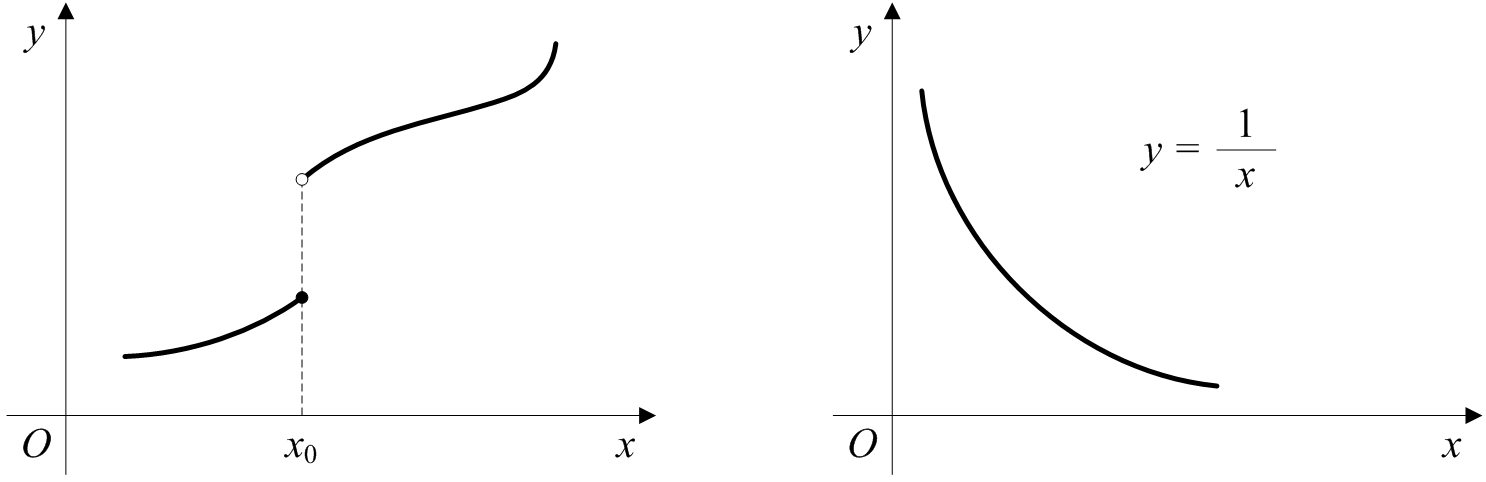
\includegraphics[height=3cm]{1.2.png}
\end{figure}

基于这个几何意义,连续的运算法则和几个定理也是非常容易理解,且不证自明。

%============================================================
\subsection{连续的运算法则}

若$f\left( x \right) ,g\left( x \right) $在点$x_0$处连续,则有
\begin{align*}
&C\cdot f\left( x \right) \\
&f\left( x \right) \pm g\left( x \right) \\
&f\left( x \right) \cdot g\left( x \right) \\
&\frac{f\left( x \right)}{g\left( x \right)}
\end{align*}
且在点$x_0$处连续。
特别注意1、2两式表明连续也是线性的。

%============================================================
\subsection{连续的定理}

\begin{theorem}[初等函数连续定理]
基本初等函数和初等函数在其定义域的区间上是连续的。
\end{theorem}

\begin{theorem}[反函数的连续性]
若函数$f\left( x \right) $在某区间内连续且单调,则其反函数$f^{-1}\left( x \right) $在原函数对应的值域内连续且单调,且具有相同的单调性。
\end{theorem}

\begin{theorem}[复合函数的连续性]
若$\underset{x\rightarrow x_0}{\lim}\varphi \left( x \right) =\varphi \left( x_0 \right) =u_0$,$\underset{u\rightarrow u_0}{\lim}f\left( u \right) =f\left( u_0 \right) $,则
\[
\underset{x\rightarrow x_0}{\lim}f\left( \varphi \left( x \right) \right) =f\left( \underset{x\rightarrow x_0}{\lim}\varphi \left( x \right) \right) =f\left( \varphi \left( x_0 \right) \right)
\]
\end{theorem}

该定理表示极限符号和函数符号可以交换顺序。
初等函数连续定理和该定理常用于计算极限。

\begin{theorem}[最值定理]
若$f\left( x \right) $在闭区间$\left[ a,b \right] $连续,则必在$\left[ a,b \right] $上有最大值和最小值。
\end{theorem}

\begin{theorem}[有界定理]
若$f\left( x \right) $在闭区间$\left[ a,b \right] $连续,则必在$\left[ a,b \right] $上有界。
\end{theorem}

\begin{theorem}[介值定理]
若$f\left( x \right) $在闭区间$\left[ a,b \right] $连续,且$f\left( a \right) \ne f\left( b \right) $,则对于任何$\forall \mu \in \left[ f\left( a \right) ,f\left( b \right) \right] $或$\forall \mu \in \left[ f\left( b \right) ,f\left( a \right) \right] $,必存在$\xi \in \left[ a,b \right] $,使得$f\left( \xi \right) =\mu $。几何上表示曲线$y=f\left( x \right) $和直线$y=\mu $至少有一个交点。
\end{theorem}

\begin{corollary}
若$f\left( x \right) $在闭区间$\left[ a,b \right] $连续,且有最大值和最小值$m,M$,则对于任何$\forall \mu \in \left[ m,M \right] $,必存在$\xi \in \left[ a,b \right] $,使得$f\left( \xi \right) =\mu $。
\end{corollary}

\begin{corollary}[根存在定理]
若$f\left( x \right) $在闭区间$\left[ a,b \right] $连续,且$f\left( a \right) \cdot f\left( b \right) <0$,则必存在$\xi \in \left[ a,b \right] $,使得$f\left( \xi \right) =0$。
\end{corollary}

\begin{corollary}[唯一根存在定理]
若$f\left( x \right) $在闭区间$\left[ a,b \right] $连续且严格单调,且$f\left( a \right) \cdot f\left( b \right) <0$,则有唯一$\xi \in \left[ a,b \right] $,使得$f\left( \xi \right) =0$。
\end{corollary}

最值定理和有界定理是等价的。

%============================================================
\subsection{两个重要的极限}

{\bf 计算$\underset{x\rightarrow 0}{\lim}\frac{\log _a\left( 1+x \right)}{x}$}

首先有
\[
\frac{\log _a\left( 1+x \right)}{x}=\log _a\left( 1+x \right) ^{\frac{1}{x}}
\]
然后运用复合函数的连续性定理:
\[
\underset{x\rightarrow 0}{\lim}\log _a\left( 1+x \right) ^{\frac{1}{x}}=\log _a\underset{x\rightarrow 0}{\lim}\left( 1+x \right) ^{\frac{1}{x}}=\log _ae=\frac{\ln e}{\ln a}=\frac{1}{\ln a}
\]
特别的,当$a=e$时:
\[
\underset{x\rightarrow 0}{\lim}\frac{\ln \left( 1+x \right)}{x}=1
\]

{\bf 计算$\underset{x\rightarrow 0}{\lim}\frac{a^x-1}{x}$}

令$a^x-1=t$,得$x=\log _a\left( t+1 \right) $,且$x\rightarrow 0$时有$t\rightarrow 0$,所以:
\[
\underset{x\rightarrow 0}{\lim}\frac{a^x-1}{x}=\underset{x\rightarrow 0}{\lim}\frac{t}{\log _a\left( t+1 \right)}=\underset{x\rightarrow 0}{\lim}\frac{1}{\log _a\left( t+1 \right) ^{1/t}}=\ln a
\]
特别的,当$a=e$时:
\[
\underset{x\rightarrow 0}{\lim}\frac{e^x-1}{x}=1
\]

\begin{tcolorbox}
该极限在求解指数函数$a^x$的导数时用到,是三大基本导数之一。
\end{tcolorbox}

%============================================================
\subsection{再论四个重要极限}

以下四个重要极限揭示了基本初等函数之间的关系:

\begin{table}[h]
\centering
\begin{tabular}{lc}
    \toprule
    极限 & 函数间的联系\\
    \midrule
    $\underset{x\rightarrow 0}{\lim}\frac{\sin x}{x}=1$ & 联系了幂函数和三角函数。\\
    $\underset{x\rightarrow \infty}{\lim}\left( 1+\frac{1}{x} \right) ^x=e$ & 联系了幂函数和指数函数。\\
    $\underset{x\rightarrow 0}{\lim}\frac{\log _a\left( 1+x \right)}{x}=\frac{1}{\ln a}$ & 联系了幂函数和对数函数。\\
    $\underset{x\rightarrow 0}{\lim}\frac{a^x-1}{x}=\ln a$ & 联系了幂函数和指数函数。\\
    \bottomrule
\end{tabular}
\end{table}




